As mentioned in Chapter.~\ref{chap:intro}, array processing serves in many different application, each with its unique requirements, setup and constraints - hence performance criteria are application dependent.
In this work, we focus on localization related applications and suggest a new architecture for the beamformer design.
Hence, to analyse the presented scheme, we use classic localization-related performance metrics.
\par
To this end, we follow the classic \cite{van2004optimum} performance analysis, elaborated in the following.
Those criteria are then used to quantify the presented architecture's performance in Chapter.\ref{chap:firstchap}.
\subsection{Beampattern}
Considering DOA estimators, the main tool for assessing an array's localization performance is expressing it's response to impinging signals with respect to the signal's DOA.
\begin{figure}
  \centering
  \begin{subfigure}[b]{0.49\linewidth}
    % 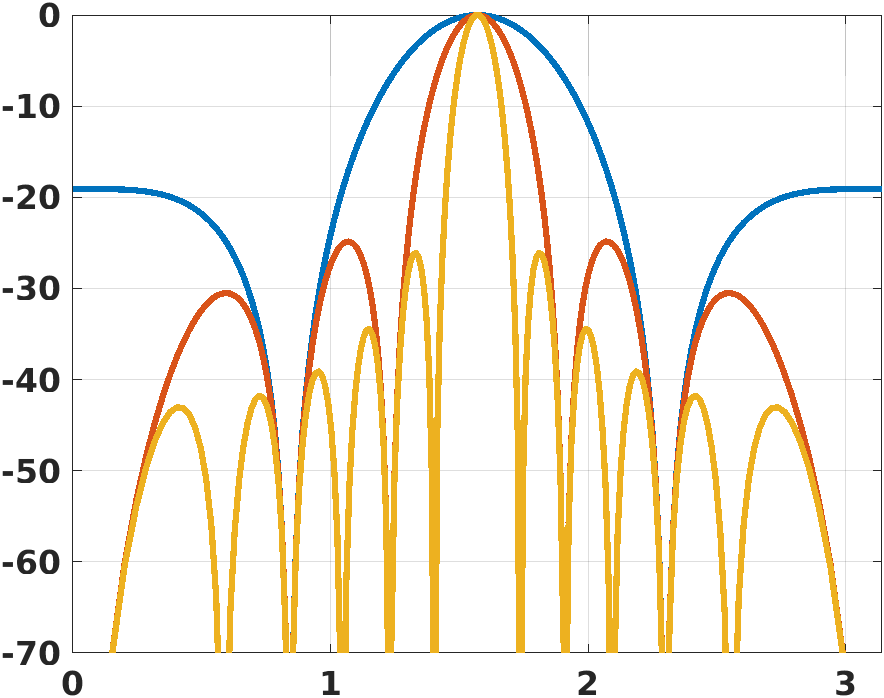
\includegraphics[width=\linewidth]{./Media/fig_commonBp_1.png}
    \begin{overpic}[width=\linewidth, 
        %grid, 
        tics=10,trim=0 0 0 0]{./Media/fig_commonBp_1.png}
            \put (19, 58){\tiny{$N\!=\!3$}}
            \put (19, 47){\tiny{$N\!=\!6$}}
            \put (19, 34){\tiny{$N\!=\!12$}}
    \end{overpic}
    \caption{}
    \label{fig_common_bps1}
  \end{subfigure}
  %
  \begin{subfigure}[b]{0.4\linewidth}
    \begin{overpic}[width=\linewidth, 
        %grid, 
        tics=10,trim=0 0 0 0]{./Media/fig_commonBp_2.png}
            \put (81, 63.5){\tiny{$N\!=\!3$}}
            \put (76, 57){\tiny{$N\!=\!6$}}
            \put (76, 53){\tiny{$N\!=\!12$}}
    \end{overpic}
    \caption{}
    \label{fig_common_bps2}
  \end{subfigure}
  \caption{Two common ways of visualizing the array's response in the 2D planar case.
  In both plots, a comparison between the conventional beamformer's responses of 3,6 and 12 elements arrays is emulated. 
  In Fig.~\ref{fig_common_bps1}, the response is presented on the $\vBrace{0,\pi}$ interval with units of dB.
  In Fig.~\ref{fig_common_bps2}, a polar plot is presented with same units for the response gain but the DOA is in degrees.}
  \label{fig_common_bps}
\end{figure}
Although for sensors in 3D space the DOA may depend on two angles (azimuth and elevation), for the sake of simplicity, we consider a planar (i.e. azimuth without elevation) DOA-only dependant array response (i.e. the \emph{beampattern})
\begin{equation}
B\rBrace{\theta} = 20\log_{10}\abs{Z\rBrace{\theta}}.
\end{equation}
The beampttern is commonly presented in a graphical manner as exemplified in Fig.~\ref{fig_common_bps}.
It's characteristics, such as main lobe width, position and attenuation of sidelobes are then analysed and compared between different schemes.
The analysis can be done theoretically, when the beampattern's mathematical expression is known or it can be conducted numerically for empirical scenarios.
% In this work, as we deal with 2D planar localization problems, we find the presentation of Fig.~\ref{fig_common_bps1} most suitable.
The DOAs of the impinging signal, may be presented in various ways where units may be degrees or radians.
% Also, as the DOA is periodical one should also choose the centering, for example when the beampattern is steered towards different angles and the author wants to center the mainlobe.
In this work, we choose to follow \cite{van2004optimum}'s $\psi$-space, i.e.
\begin{equation}
    \psi\rBrace{\theta_{d}}=\frac{2\pi}{\lambda}\cos{\theta_{d}}\cdot{}d,
\end{equation}
where $\lambda$ is the impinging signal's wavelength.
The reader may notice that $\psi$ is exactly the electric phase $\theta$ defined in \eqref{eq:thetaULA} therefore, throughout the rest of the work, we use the $\theta$ notation. 
Also, we choose to plot beampatterns using $\Delta\theta = \theta\rBrace{\theta_{d}} - \theta\rBrace{\theta_{s}}$, where $\theta_{s}$ is the steering angle of the array, for it centers the mainlobe, enabling convenient comparison.
\subsection{The normalized beampattern}
As the absolute output gain is system dependent, comparing two different beampatterns is not possible where their maximal gain of the mainlobe are different.
Therefore, a common practice \cite{van2004optimum} when analysing the array's spatial performance, is to normalize the beampattern such that the mainlobe's output gain at it's peak is 1 (0dB), thus enabling convenient comparable measures extraction.
This quantity will be referred to as $\mathcal{H}$.
\subsection{Half power beamwidth}
% Considering localization problems, possibly the main interest is spatial resolution, related to localization accuracy and distinction of spatially close objects, where ``close`` can be interpreted as small physical distance between objects of interest or objects that may be physically distant from each other but from the array's perspective are in relatively similar.
% \par
Considering localization problems, the spatial resolution is obviously linked to the main lobe's width, i.e. higher resolution is achieved for narrower main lobe.
The Half Power BeamWidth (HPBW), marked as $\Delta\theta_{HPBW}$, is defined to be the 3-dB beamwidth, i.e. the point where $\abs{B\rBrace{\theta}}^{2} = 0.5$ or $\abs{B\rBrace{\theta}} = 1/\sqrt{2}$.
For standard ULA, assuming large $N$ values, it is known \cite{van2004optimum} that
\begin{equation}
    \label{eq_known_HBPW}
    \dThetaHPBW/2= 1.4/N.
\end{equation}
\par
Obviously, we aim to show that the presented architecture increases the resolution, comparing to other arrays by proving that the beamwidth shrinks.
%
%
%
\subsection{Sidelobes attenuation}
% As the beampattern consists of multiple harmonics (as the number of elements $N$), sidelobes occur when the some harmonics are summed, showing as peaks other than the mainlobe.
% As this is an unwanted result, the height and their rate of decrease are measured aiming to prefer arrays where their height is reduced and the decrease rate is increased.
A known \cite{van2004optimum} parasitic phenomenon of beampatterns is sidelobes, which manifests as energy peaks outside the mainlobe, typically highest near the mainlobe and decreasing towards the deges of the beampattern.
In the context of localization, this can cause false detection or reduction in spatial resolution.
Related spatial performance metrics are the sidelobes gain and rate of decrease
%
%
%
\subsection{Directivity}
A common measure of performance of an array or aperture is the directivity $\mathcal{D}$.
As in \cite{van2004optimum}, in a transmitting array or aperture, $\mathcal{D}$ represents the maximum radiation intensity (power per DOA) divided by the average radiation intensity (averaged over all DOAs).
Also, in a receiving antenna, the denominator represents the noise power at the array (or aperture) output due to isotropic noise (noise distributed uniformly over all DOAs). 
The numerator will represent the power due to a signal arriving from a certain DOA ($\theta_{T}$) - Thus, $\mathcal{D}$ can be interpreted as the array gain against isotropic noise.
We define the power pattern, $P\rBrace{\theta_{d}}$, to be the squared magnitude of the beampattern $B\rBrace{\theta_{d}}$
\begin{equation}
    P\rBrace{\theta_{d}} = \abs{B\rBrace{\theta_{d}}}^{2}
\end{equation}
where the frequency dependence is suppressed.
Then the directivity $\mathcal{D}$ is defined as
\begin{equation}\label{eq_D}
    \mathcal{D}\rBrace{\theta_{T}} = \frac{
    P\rBrace{\theta_{T}}
    }{
    \frac{1}{2\pi}\int_{0}^{2\pi}P\rBrace{\theta}d\theta
    }
\end{equation}
In the following, as we consider steered (to $\theta_{s}$) arrays, we suppress the DOA dependency such that $\mathcal{D} = \mathcal{D}\rBrace{{\theta_{s}}}$. 
For uniformly weighted ULAs with no feedback, it is known \cite{van2004optimum} that $\mathcal{D} = N$.
